\documentclass{article}

\usepackage[utf8]{inputenc}
\usepackage[brazilian]{babel}
\usepackage{graphicx}
\usepackage{float}
\usepackage[pdftex]{hyperref}
\usepackage{epstopdf}
\usepackage{etoolbox}
\usepackage{amsmath}
\usepackage{amsfonts}
\usepackage{amssymb}
\usepackage{caption}
\usepackage{subcaption}
\usepackage{setspace}
\usepackage{tikz}

\patchcmd{\thebibliography}{\section*}{\section}{}{}
\newcommand{\R}{\ensuremath{\mathbb{R}}}
\newcommand{\Prob}{\ensuremath{\mathbb{P}}}
\newcommand{\K}{\ensuremath{\mathbb{K}}}
\newcommand{\U}{\ensuremath{\mathbb{U}}}
\newcommand{\N}{\ensuremath{\mathbb{N}}}
\newcommand{\Lg}{\ensuremath{\mathbb{L}}}
\newcommand{\T}{\ensuremath{\rm Tr}}
\newcommand{\sg}{{\sigma(x_k)}}

\newcommand{\G}{\ensuremath{\mathcal{G}}}
\newcommand{\F}{\ensuremath{\mathcal{F}}}
\newcommand{\C}{\ensuremath{\mathcal{C}}}
\newcommand{\E}{\ensuremath{\mathcal{E}}}
\newcommand{\Hn}{\ensuremath{\mathcal{H}}}
%\newcommand{\Hoo}{\ensuremath{\mathcal{H}_\infty}}
\newcommand{\Hop}{\ensuremath{\mathcal{H}_{op}}}
% --------------------------------------------------
\newtheorem{theo}{Teorema}
\newtheorem{exa}{Exemplo}
\newtheorem{lemm}{Lema}
\newtheorem{coro}{Corolário}
\newtheorem{defn}{Definição}[section]

%opening


\begin{document}

\begin{titlepage}
\begin{center}

\newcommand{\HRule}{\rule{\linewidth}{0.5mm}}
% Upper part of the page. The '~' is needed because \\
% only works if a paragraph has started.

\includegraphics[width=0.15\textwidth]{logounicamp.pdf}~\\[1cm]

\textsc{\LARGE Universidade Estadual de Campinas}\\[1.5cm]

\textsc{\Large Faculdade de Engenharia Mecânica}\\[0.5cm]

% Title
\HRule \\[0.4cm]
{ \huge \bfseries ES828 - Laboratório de Controle de Sistemas\\ \vspace{1cm} Relatório - Experimento 2 \\
\Large{Método de identificação de plantas eletrônicas} \\[0.4cm] }

\HRule \\[1.5cm]

% Author and supervisor
\begin{minipage}{0.6\textwidth}
\begin{flushleft} \large
\emph{Nome:}\\
Daniel Dello Russo Oliveira\\ Marcelli Tiemi Kian
\end{flushleft}
\end{minipage}
\begin{minipage}{0.2\textwidth}
\begin{flushright} \large
\emph{RA}\\ 101918\\
117892
\end{flushright}
\end{minipage}

\vfill

% Bottom of the page
{\large \today}

\end{center}
\end{titlepage}


\onehalfspacing
\section{Objetivos} 
O objetivo desse experimento foi o projeto e análise de um controlador via realização em espaço de estado e um observador de estado para a planta eletrônica identificada no experimento 2\cite{bb:lab2}. 
	
\section{Projeto do Controlador}
Como nossa planta apresentou problemas durante o decorrer do experimento, apresentando respostas diferentes para o mesmo controlador de acordo com a temperatura do circuito e a posição em que o mesmo se encontrava (provavelmente devido a componentes defeituosos e mal contatos), nós refizemos o experimento utilizando a planta número 8, conforme sugerido pela professora.
Essa planta teve sua função de transferência, representada pela equação \ref{eq:gs}, calculada por outro grupo usando as medidas realizadas durante o experimento 2 e nós, através do seu relatório\cite{bb:lab2gui}, recuperamos esses valores e utilizamos a mesma metodologia utilizada no pré relatório \cite{bb:prelab6} para o projeto do controlador e observador em espaço de estado conforme a figura \ref{fig:contrss}, com as matrizes $A$, $B$ e $C$ indicadas em \ref{eq:mata}, \ref{eq:matb} e \ref{eq:matc}.\\

\begin{equation}
\label{eq:gs}
G(s) = \frac{\kappa_1\kappa_2\kappa_3\kappa_4}{(s\tau_2 + 1)(s\tau_3 + 1)s} = \frac{29800}{s^3 + 120 s^2 + 3316 s}
\end{equation}

\begin{table}[H]
	\centering
	\caption{Parâmetros numéricos da função de transferência}
	\label{tab:valores}
	\begin{tabular}{|c|c|}
		\hline Parâmetro & Valor \\ 
		\hline $\kappa_1$ & $-0.0995$\\ 
		\hline $\kappa_2$ & $-2.1626$\\ 
		\hline $\kappa_3$ & $-4.5739$\\ 
		\hline $\kappa_4$ & $-9.1333$\\ 
		\hline $\tau_2$ & $0.0130$\\ 
		\hline $\tau_3$ & $0.0232$ \\ 	
		\hline 
	\end{tabular} 
\end{table}

\begin{figure}[H]
	\centering
	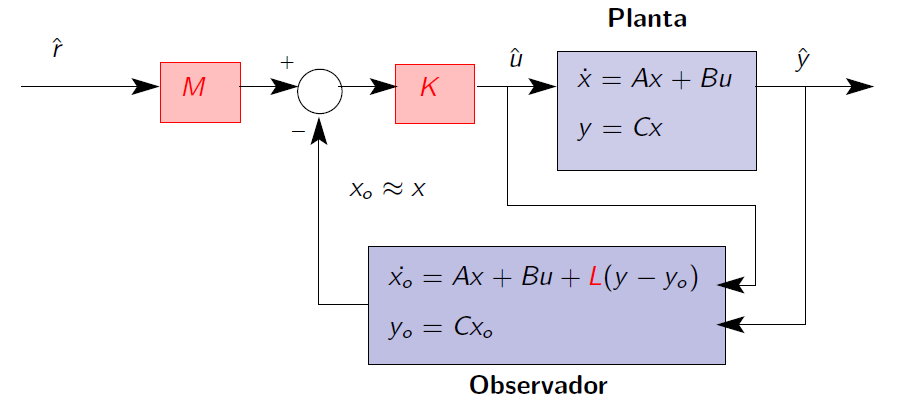
\includegraphics[width=0.8\linewidth]{contrss}
	\caption{Diagrama de blocos do sistema}
	\label{fig:contrss}
\end{figure}

\begin{equation}
\label{eq:mata}
A=
\begin{bmatrix}
 0 & 1 & 0 \\
 0 & 0 & 1 \\
 0 & -\frac{1}{\tau_2\tau_3} & -\frac{\tau_2+\tau_3}{\tau_2\tau_3}
\end{bmatrix} = 
\begin{bmatrix}
0 & 1 & 0 \\
0 & 0 & 1 \\
0 & -3315.65 & -120.03
\end{bmatrix}
\end{equation}
\begin{equation}
\label{eq:matb}
B=
\begin{bmatrix}
0 \\
0 \\
\frac{\kappa_1\kappa_2\kappa_3\kappa_4}{\tau_2\tau_3}
\end{bmatrix} = 
\begin{bmatrix}
0 \\
0 \\
29804.5
\end{bmatrix}
\end{equation}
\begin{equation}
\label{eq:matc}
C=
\begin{bmatrix}
1 & 0 & 0
\end{bmatrix}
\end{equation}

Com essas matrizes e as especificações do projeto, listadas a seguir projetamos o controlador:
\begin{itemize}
	\item Tempo de estabilização de aproximadamente $0.5$ [s].
	\item Fator de amortecimento igual a $\sqrt{2}/2$.
	\item Polo em $s=-30$.
	\item Erro em regime permanente nulo a uma entrada rampa.
	\item Amplitude do sinal de controle não pode ultrapassar $\pm10$ [Volts].
\end{itemize}\
 Determinamos as matrizes K, L e M para a implementação do sistema conforme detalhado no pré relatório \cite{bb:prelab6}, porém alteramos os autovalores desejados para o observador de maneira a aumentar sua velocidade de resposta. Definimos que esses novos autovalores deveriam ser da ordem de 5 vezes maiores que o maior autovalor do controlador ( $-30$), logo escolhemos o valor $-150$ com multiplicidade 3. Obtivemos as matrizes \ref{eq:matk}, \ref{eq:matl} e \ref{eq:matm}.
\begin{equation}
\label{eq:matk}
K=
\begin{bmatrix}
0.1232 & -0.0914 & -0.0025
\end{bmatrix}
\end{equation}

\begin{equation}
\label{eq:matl}
L=
\begin{bmatrix}
329.97 & 24578.78 & -669182.13
\end{bmatrix}
\end{equation}

\begin{equation}
\label{eq:matm}
M = \frac{\frac{s}{5.142} + 1}{\frac{s}{30} + 1}*
\begin{bmatrix}
1\\
0.5\\
-18.31
\end{bmatrix}
\end{equation}

\subsection{Implementação}
Para realizar o sistema, seguimos a estrutura recomendada no roteiro\cite{bb:roteiro}, obtendo a implementação mostrada na figura \ref{fig:impl} com as funções de transferência \ref{eq:hs}, \ref{eq:cus} e \ref{eq:cys}.
\begin{figure}[H]
	\centering
	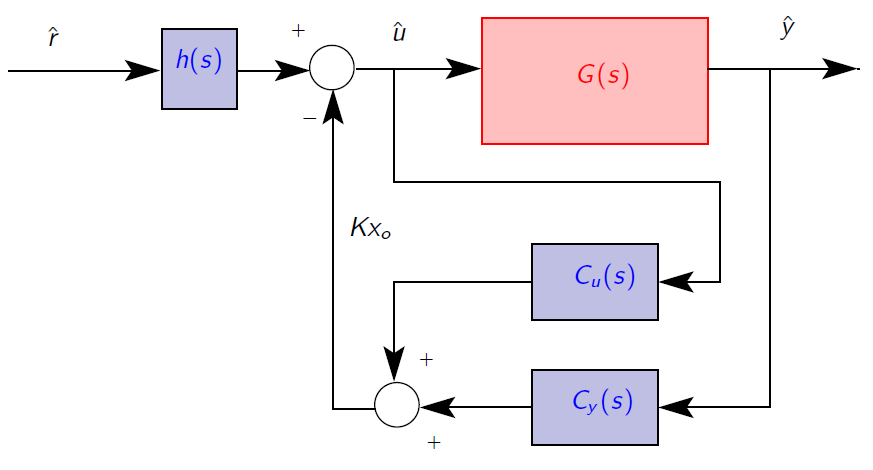
\includegraphics[width=0.8\linewidth]{impl}
	\caption{Diagrama de blocos da implementação final do controle}
	\label{fig:impl}
\end{figure}

\begin{equation}
\label{eq:hs}
h(s) = KM(s) = \frac{0.719 s + 3.697}{s+30}
\end{equation}
\begin{equation}
\label{eq:cus}
C_u(s) = K(sI - (A - LC))^{-1}B = \frac{-74.38 s^2 - 27270 s - 2723000}{s^3 + 450 s^2 + 67500 s + 3375000}
\end{equation}
\begin{equation}
\label{eq:cys}
C_y(s) = K(sI - (A - LC))^{-1}L = \frac{-535.6 s^2 + 2834 s + 415900}{s^3 + 450 s^2 + 67500 s + 3375000}
\end{equation}


\section{Simulação}
Com o auxílio do Simulink simulamos (com e sem ruído branco) para esse novo controlador e planta as respostas do controlador a uma onda quadrada de amplitude $1V$ e frequência de $0,25Hz$, e seus esforços de controle, que podem ser vistas nas figuras \ref{fig:yur} e \ref{fig:yurN}.
\begin{figure}[H]
	\centering
	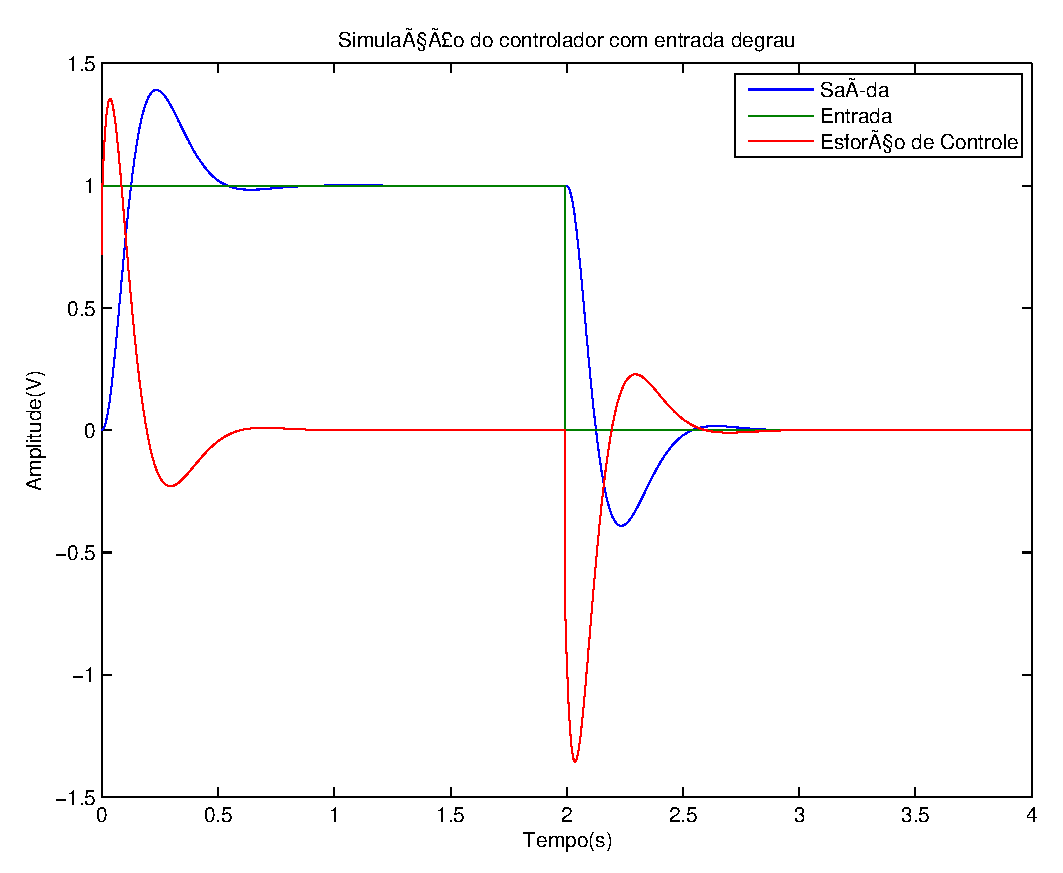
\includegraphics[width=0.8\linewidth]{../yur}
	\caption{Resposta e esforço de controle simulados para onda quadrada}
	\label{fig:yur}
\end{figure}
\begin{figure}[H]
	\centering
	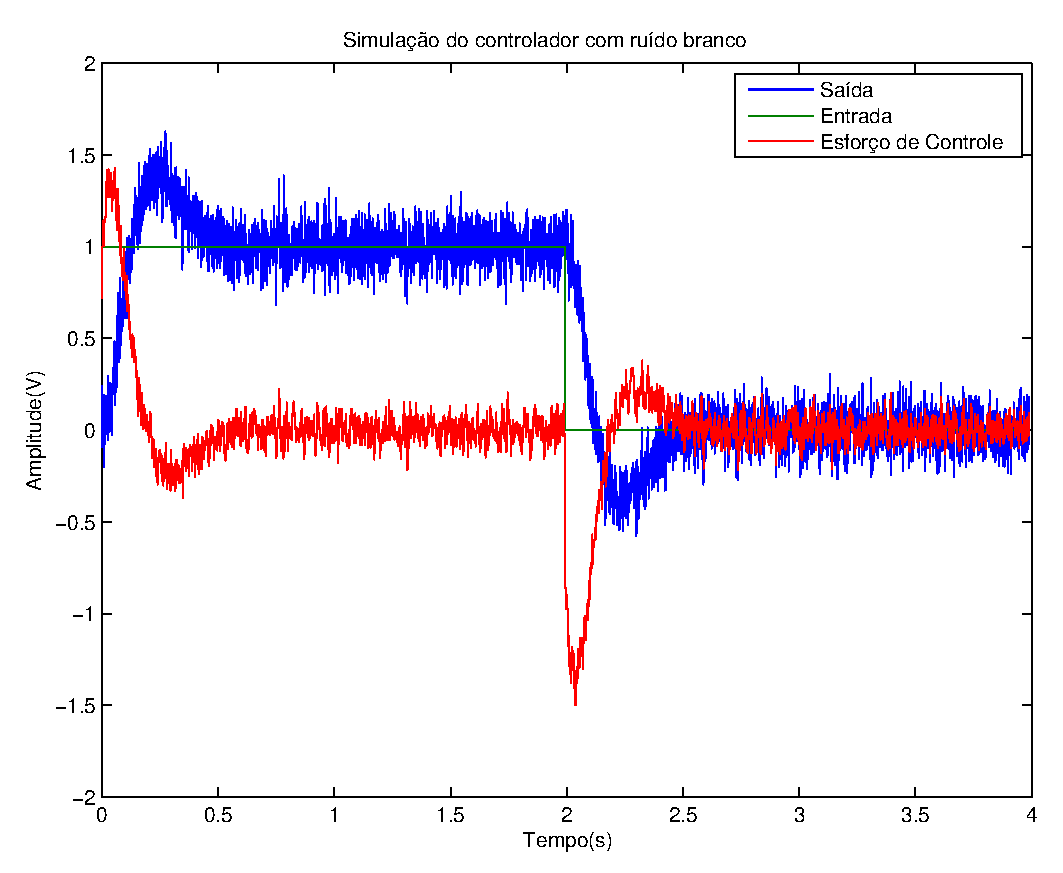
\includegraphics[width=0.8\linewidth]{../yurN}
	\caption{Resposta e esforço de controle simulados para onda quadrada, com ruído branco}
	\label{fig:yurN}
\end{figure}

Para analisar a eficiência do nosso observador, simulamos o modelo no espaço de estados (em torno do ponto de equilíbrio [0,0,0]', com estado inicial do controlador [0, 0, 0]' e do observador [1, 0, 0]') e plotamos o estado do sistema e o estado estimado pelo observador, que podem ser vistos nas figuras \ref{fig:obsx1}, \ref{fig:obsx2} e \ref{fig:obsx3}.
\begin{figure}[H]
	\centering
	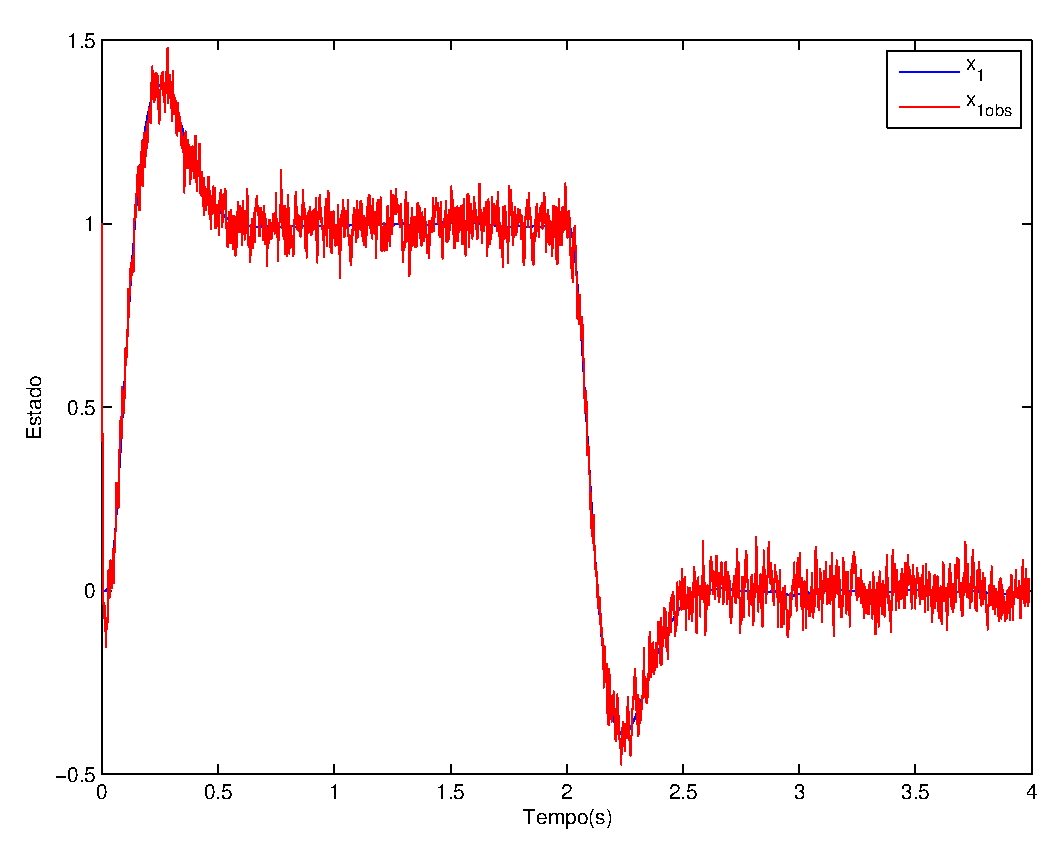
\includegraphics[width=0.8\linewidth]{../obsx1}
	\caption{Estado $x_1$ real e estimado do sistema simulado para onda quadrada, com ruído branco}
	\label{fig:obsx1}
\end{figure}
\begin{figure}[H]
	\centering
	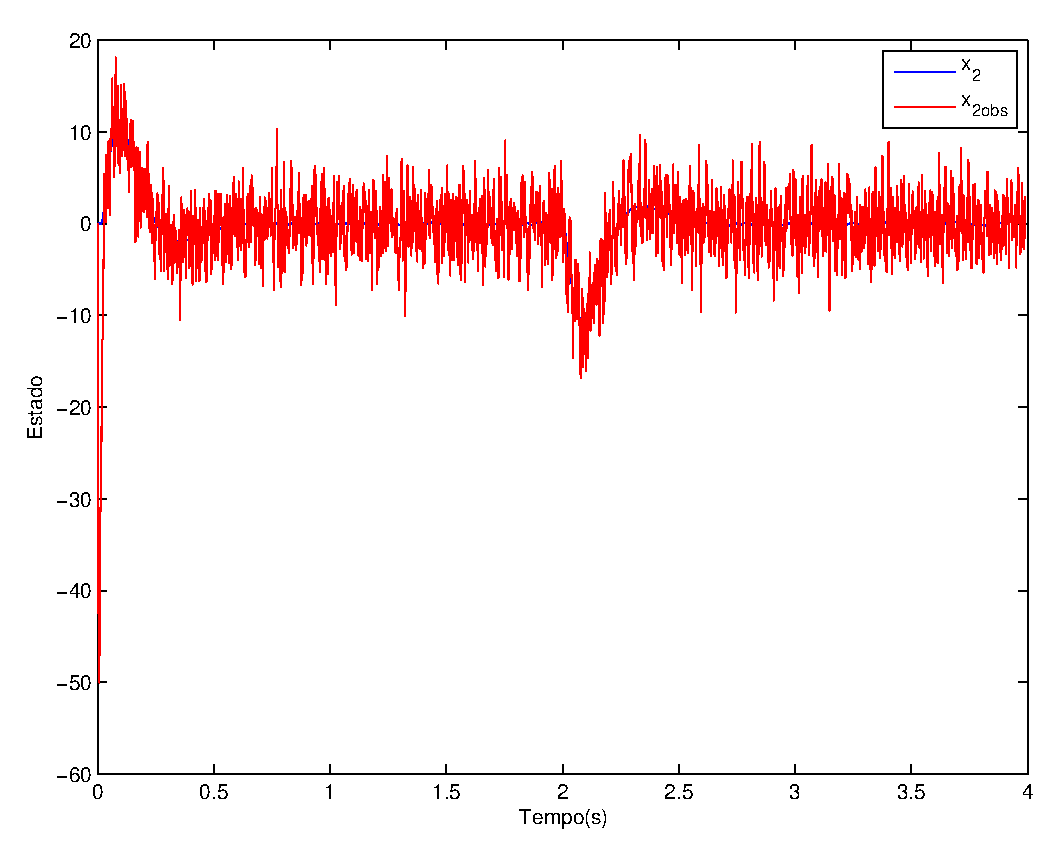
\includegraphics[width=0.8\linewidth]{../obsx2}
	\caption{Estado $x_2$ real e estimado do sistema simulado para onda quadrada, com ruído branco}
	\label{fig:obsx2}
\end{figure}
\begin{figure}[H]
	\centering
	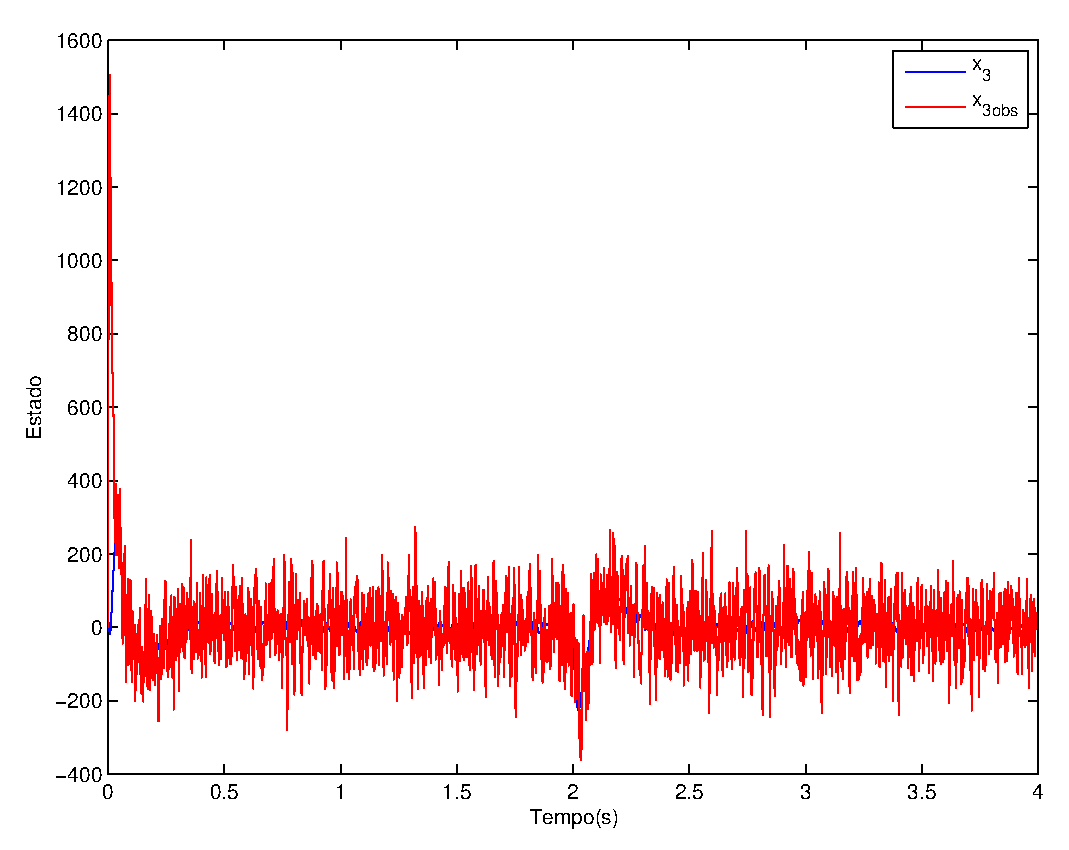
\includegraphics[width=0.8\linewidth]{../obsx3}
	\caption{Estado $x_3$ real e estimado do sistema simulado para onda quadrada, com ruído branco}
	\label{fig:obsx3}
\end{figure}
Como podemos ver o observador projetado segue bem o sistema real e não foi gravemente afetado pelo ruído.

Simulamos também a resposta deste controlador a uma rampa, mostrada na figura \ref{fig:yurR}. Como podemos ver, o erro estacionário para essa entrada é nulo, conforme desejado.
\begin{figure}[H]
	\centering
	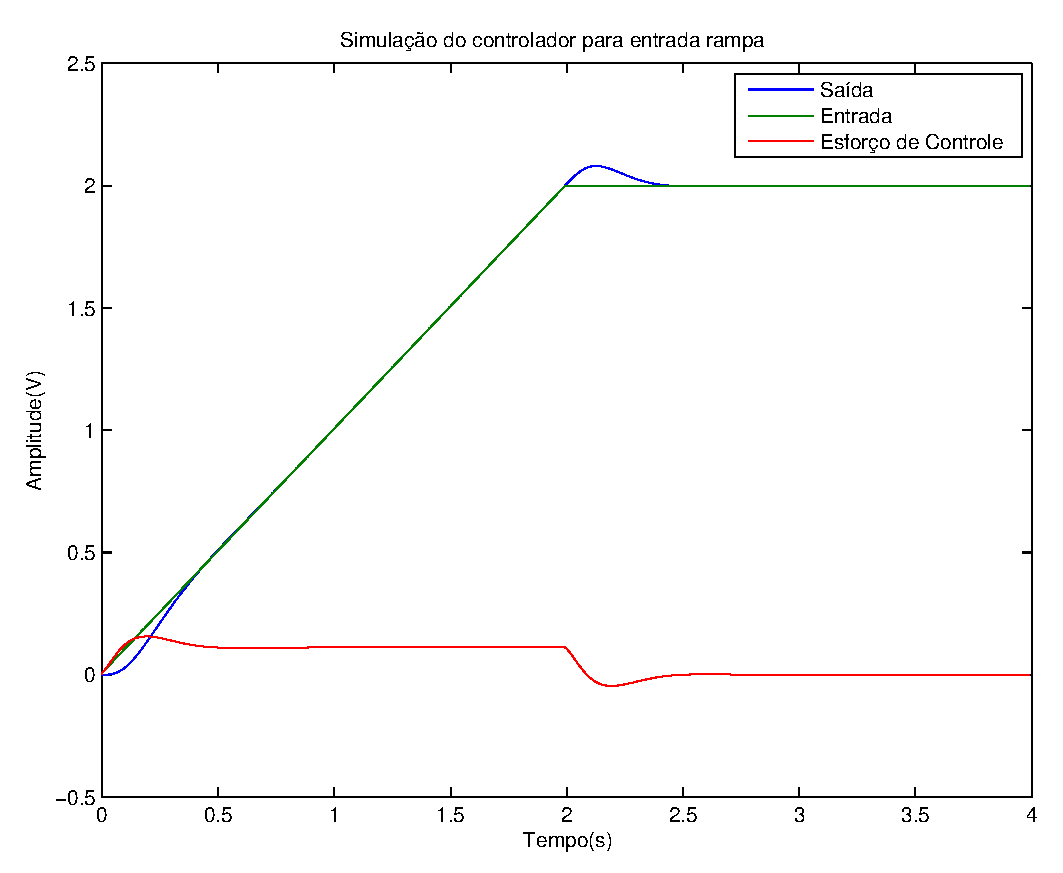
\includegraphics[width=0.8\linewidth]{../yurR}
	\caption{Resposta e esforço de controle simulados para rampa}
	\label{fig:yurR}
\end{figure}
A tabela \ref{tab:stepinfo} apresenta as características da resposta desse controlador simulado, obtida com o auxílio da função \textit{stepinfo} do Matlab.
\begin{table}[H]
	\centering
	\caption{Características da resposta do controlador simulado}
	\label{tab:stepinfo}
	\begin{tabular}{|c|c|}
		\hline Sobrelevação 				& $39.1095\%$ \\ 
		\hline Tempo de estabilização 		& $0.5089$ [s]\\ 
		\hline Tempo de subida				& $0.0835$ [s]\\ 
		\hline Erro estacionário (degrau) 	& $0$\\ 
		\hline Erro estacionário (rampa) 	& $0$\\ 
		\hline 
	\end{tabular} 
\end{table}

Como podemos ver o sistema atinge todas as especificações e não é muito susceptível a ruídos, porém ele apresenta uma sobrelevação bastante significativa. Nossa análise mostra que essa sobrelevação está associada à matriz M, porque quando relaxamos o critério de erro estacionário à rampa observa-se uma diminuição do overshoot para $5\%$.

Isso acontece pois essa matriz acrescenta um zero (em $- 5.142$) no sistema somando um termo derivativo à resposta original, o que causa um aumento na sobrelevação e uma aceleração na resposta do sistema.

\section{Análise dos Resultados}
Seguindo a metodologia descrita no roteiro \cite{bb:roteiro}, implementamos o sistema planta-controlador digital e medimos sua resposta a uma onda quadrada de amplitude de $1V$ e frequência de $0.25Hz$ com o auxílio do LabView e da plataforma de desenvolvimento Elvis que pode ser vista na figura \ref{fig:yrSIS} e seu esforço de controle que pode ser visto na figura \ref{fig:urSIS}.

\begin{figure}[H]
	\centering
	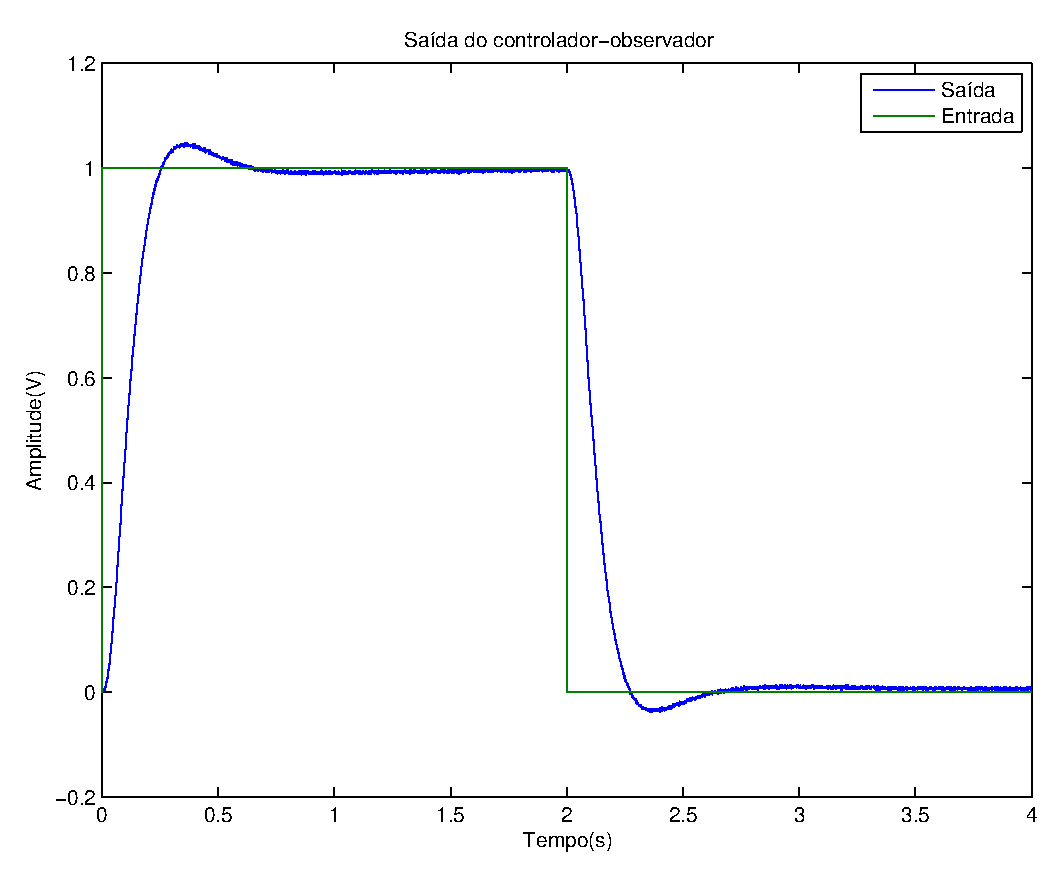
\includegraphics[width=0.8\linewidth]{../yrSIS}
	\caption{Resposta do sistema para onda quadrada}
	\label{fig:yrSIS}
\end{figure}
\begin{figure}[H]
	\centering
	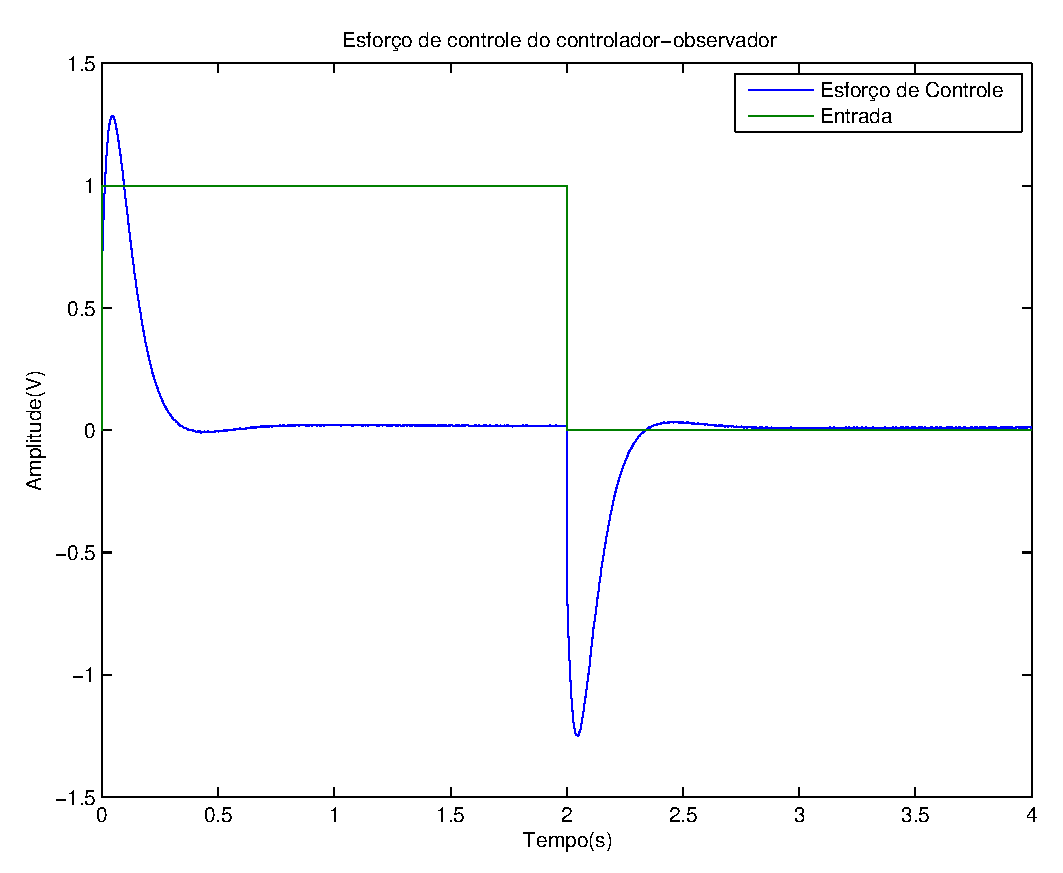
\includegraphics[width=0.8\linewidth]{../urSIS}
	\caption{Esforço de controle do sistema para onda quadrada}
	\label{fig:urSIS}
\end{figure}

Ao integrar à resposta ao degrau mostrada acima, obtemos uma estimativa da resposta à rampa desse controlador que pode ser vista na figura \ref{fig:yrSISR}.
\begin{figure}[H]
	\centering
	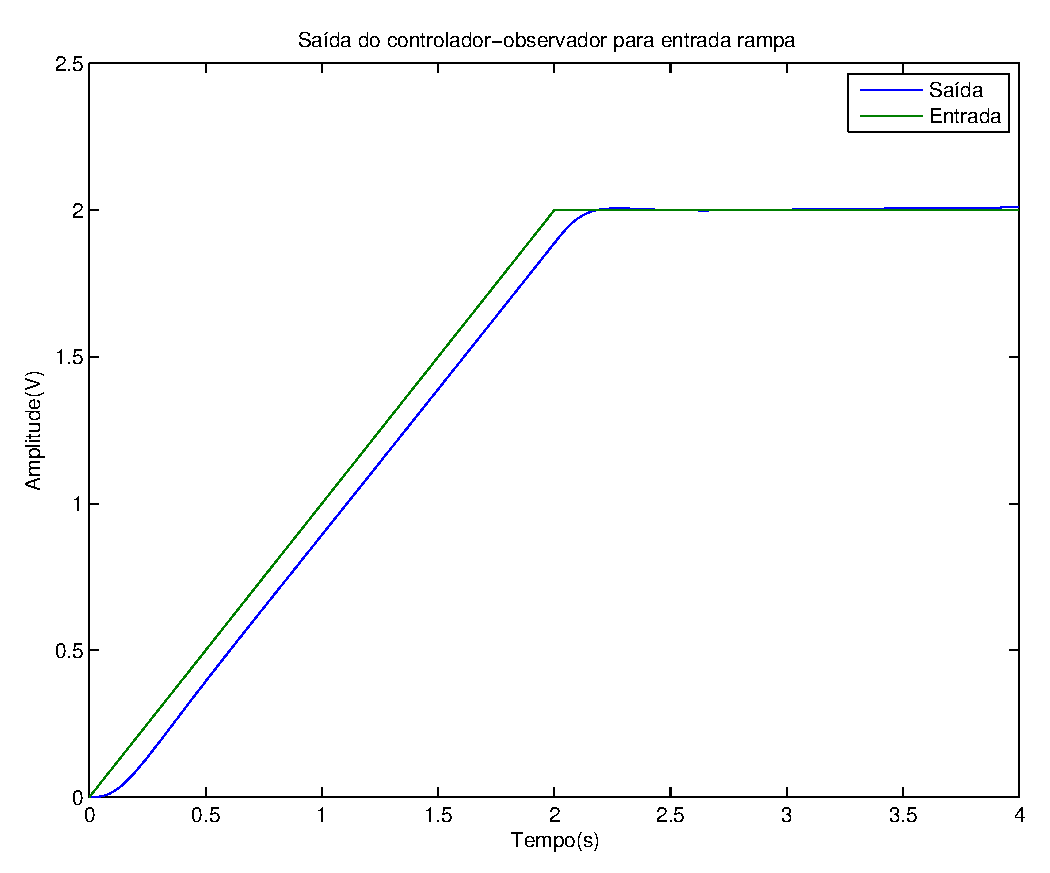
\includegraphics[width=0.8\linewidth]{../yrSISR}
	\caption{Resposta do sistema à rampa}
	\label{fig:yrSISR}
\end{figure}

A tabela \ref{tab:stepinfoSIS} apresenta as características da resposta desse controlador, obtida com o auxílio da função \textit{stepinfo} do Matlab.
\begin{table}[H]
	\centering
	\caption{Características da resposta do controlador}
	\label{tab:stepinfoSIS}
	\begin{tabular}{|c|c|}
		\hline Sobrelevação 				& $39.1095\%$ \\ 
		\hline Tempo de estabilização 		& $0.5089$ [s]\\ 
		\hline Tempo de subida				& $0.0835$ [s]\\ 
		\hline Erro estacionário (degrau) 	& $0$\\ 
		\hline Erro estacionário (rampa) 	& $0$\\ 
		\hline 
	\end{tabular} 
\end{table}
Como podemos ver a resposta obtida é diferente da simulada, isso se deve provavelmente às diferenças entre a planta real e a calculada. 

%TODO COMENTAR
\section{Comparação com os outros controladores}

Mesmo tratando-se de plantas diferentes, comparamos os resultados desse controlador com os projetados nos laboratórios anteriores. Como as duas plantas tem uma função de transferência bastante próxima esperamos que os resultados apresentem alguma significância. Devemos ressaltar porém que a planta $8$ tem um de seus polos nas proximidades de $-77$, enquanto a planta $6$ tinha o mesmo polo próximo a $-48$, logo a planta em que o controlador-observador foi implementado é mais rápida.

Podemos ver na figura \ref{eq:yrcomp} a comparação entre esse controlador e os melhores controladores dos laboratórios anteriores: os controladores digitais proporcional com sobrelevação de 2\% e PID projetado pelo método Ziegler-Nichols do experimento 3 \cite{bb:lab3}, o controlador PID analógico do experimento 4 \cite{bb:lab4} e o controlador avanço-atraso do experimento 5 \cite{bb:lab5}.
\begin{figure}[H]
	\centering
	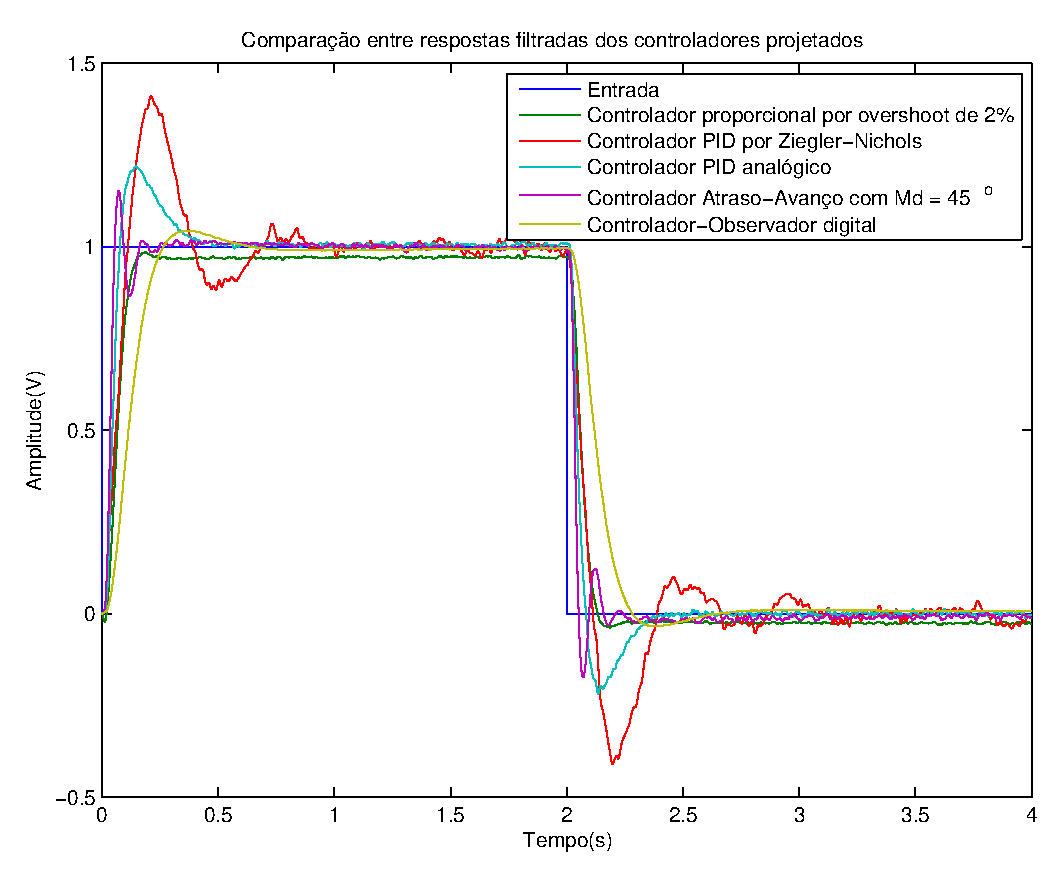
\includegraphics[width=0.8\linewidth]{../yfrcomp}
	\caption{Comparação entre as respostas filtradas dos controladores para onda quadrada}
	\label{fig:yrcomp}
\end{figure}

%TODO: COMENTAR ISSO


\begin{thebibliography}{widestlabel}
	\bibitem{bb:roteiro}{Roteiro do experimento disponibilizado para os alunos}
	\bibitem{bb:lab2}{KIAN, Marcelli; OLIVEIRA, Daniel. \textit{Relatório - Experimento 2:} Identificação de plantas eletrônicas.}
	\bibitem{bb:lab2gui}{DAVID, Vinícius; GARCIA, Augusto; SOUZA, Guilherme. \textit{Relatório - Experimento 2:} Identificação de plantas eletrônicas.}
	\bibitem{bb:lab3}{KIAN, Marcelli; OLIVEIRA, Daniel. \textit{Relatório - Experimento 3:} Controle de plantas eletrônicas utilizando um controlador PID digital.}
	\bibitem{bb:lab4}{KIAN, Marcelli; OLIVEIRA, Daniel. \textit{Relatório - Experimento 4:}  Controle de plantas eletrônicas utilizando um controlador PID analógico.}
	\bibitem{bb:lab5}{KIAN, Marcelli; OLIVEIRA, Daniel. \textit{Relatório - Experimento 5:}  Controle de plantas eletrônicas utilizando um controlador atraso-avanço digital.}
	\bibitem{bb:prelab6}{KIAN, Marcelli; OLIVEIRA, Daniel. \textit{Pré Relatório - Experimento 6:} Controle por realimentação de saída de uma planta eletrônica.}
\end{thebibliography}
\end{document}

